\section{Passo 10 — Indicadores descritivos}
\label{sec:passo10}

\subsection*{Objetivo}
Descrever o corpus por período, jurisdição, concentração de titularidade, depositantes, inventores,
classificação, anterioridade e citações.

\begin{figure}[H]
\centering
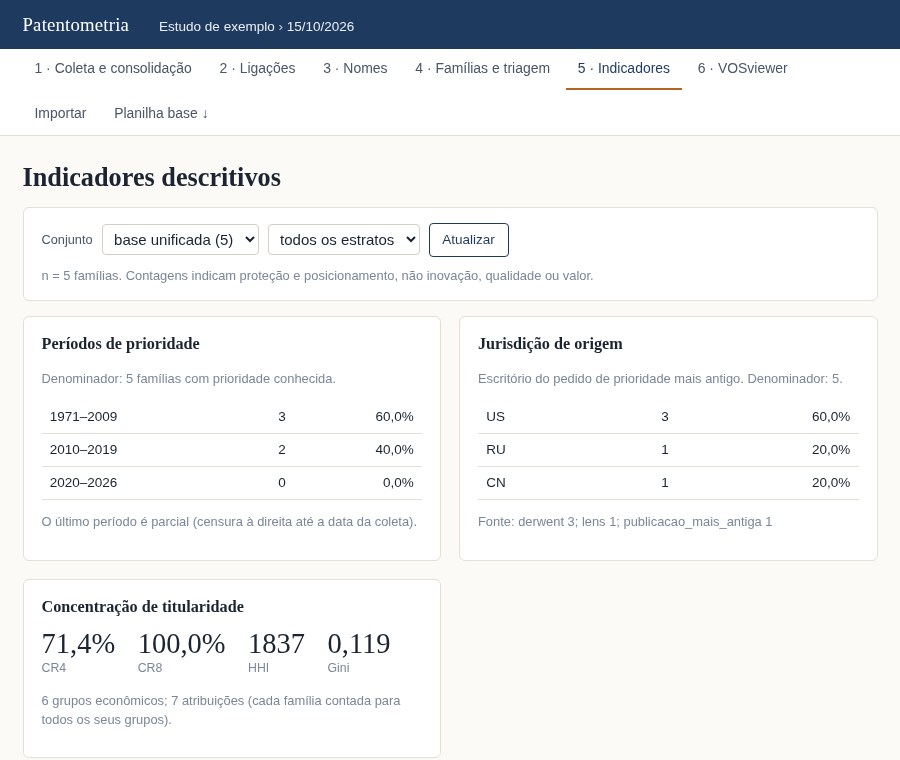
\includegraphics[width=0.92\linewidth]{img/12_indicadores_1.png}
\caption{Indicadores: períodos de prioridade, jurisdição de origem e concentração de titularidade.
Todos os cartões informam o denominador.}
\label{fig:ind1}
\end{figure}

\begin{figure}[H]
\centering
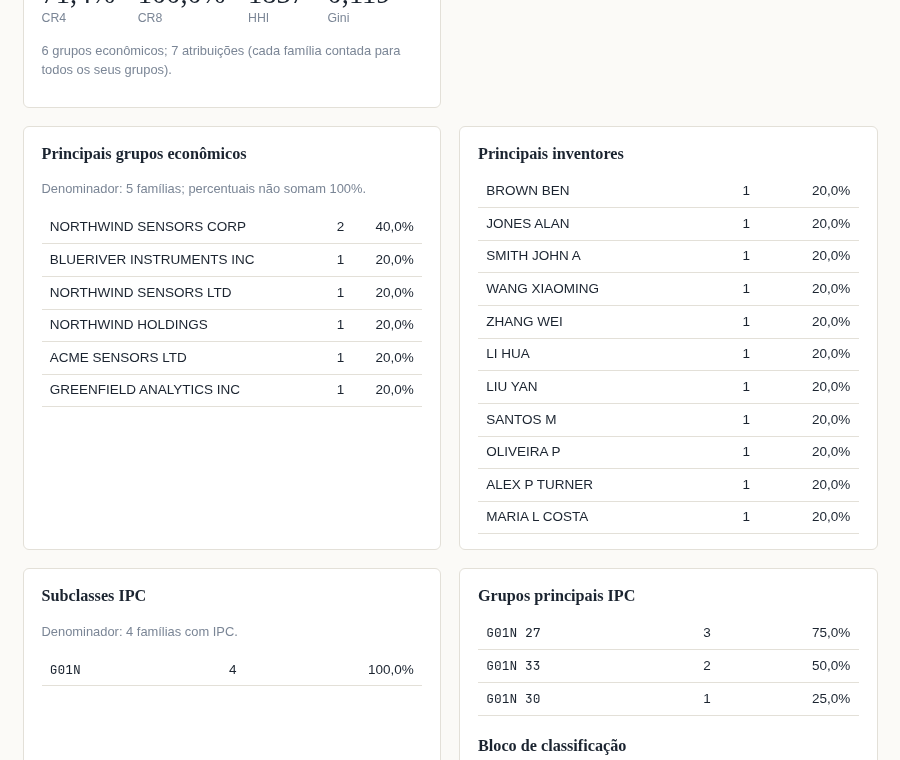
\includegraphics[width=0.92\linewidth]{img/12_indicadores_2.png}
\caption{Depositantes, grupos econômicos e inventores, com o número de famílias e de atribuições.}
\label{fig:ind2}
\end{figure}

\begin{figure}[H]
\centering
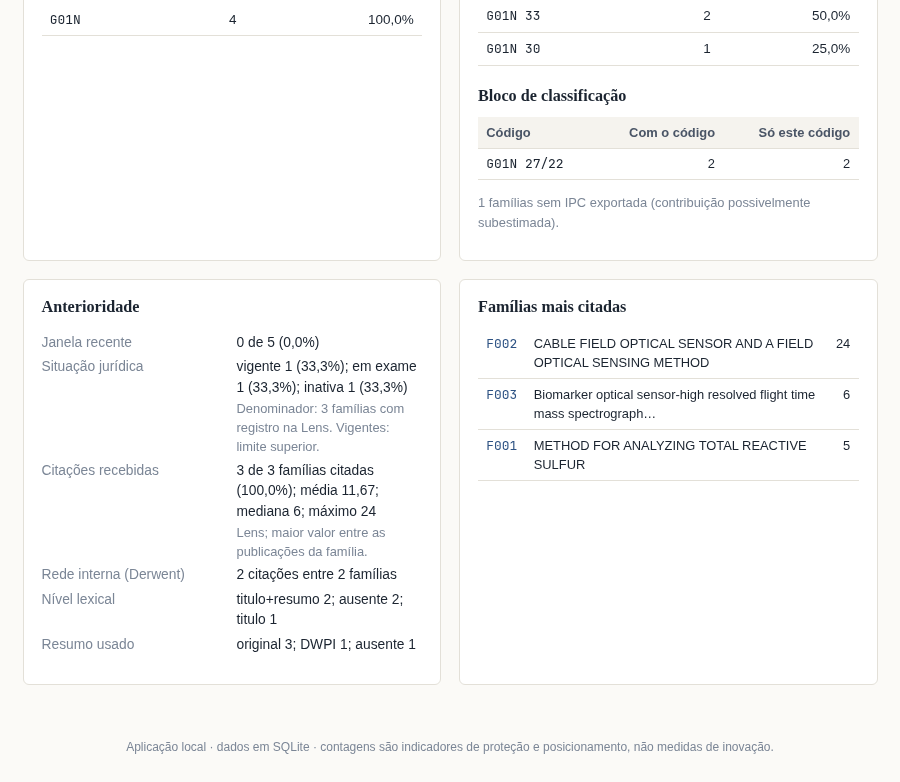
\includegraphics[width=0.92\linewidth]{img/12_indicadores_3.png}
\caption{Classificação IPC, anterioridade e famílias mais citadas.}
\label{fig:ind3}
\end{figure}

\subsection*{O que fazer}
\begin{enumerate}
\item Abra \textbf{Indicadores} e escolha o conjunto: \emph{base unificada} ou \emph{base final}.
\item Escolha o estrato (todos, S1, S2).
\item Leia cada cartão começando pelo denominador; só depois compare os valores.
\item Exporte a planilha base (Passo 12) para guardar os números com a data da coleta.
\end{enumerate}

\subsection*{Como interpretar}
\textbf{Períodos.} Na demonstração, 3 famílias (60\%) têm prioridade entre 1971 e 2009, 2 (40\%) entre
2010 e 2019 e nenhuma entre 2020 e 2026. O último período é parcial: a censura à direita faz qualquer
queda parecer maior do que é.

\textbf{Jurisdição.} Conta o escritório da prioridade mais antiga: EUA 3 (60\%), Rússia 1, China 1. É
um indicador de onde a proteção foi pedida primeiro, não de onde o mercado é maior.

\textbf{Concentração.} CR4 = 71,4\%, CR8 = 100\%, HHI = 1.837 e Gini = 0,119, sobre 6 grupos
econômicos e 7 atribuições. CR4 e CR8 medem a fatia dos maiores; HHI cresce quando poucos concentram;
Gini mede desigualdade na distribuição. Com cinco famílias, esses valores são instáveis: um único
documento muda o resultado. Use-os para descrever o corpus, não para afirmar estrutura de mercado.

\textbf{Depositantes e inventores.} O número entre parênteses é de famílias; a soma das atribuições
pode exceder o total de famílias porque uma família pode ter vários titulares. Compare sempre com o
total informado no rodapé do cartão.

\textbf{IPC.} Uma família pode ter várias classificações; por isso a soma das classes não fecha com o
número de famílias. A classe principal é a mais frequente, não a única.

\textbf{Anterioridade.} Mostra o tempo entre a prioridade e a publicação (ou a coleta). Serve para
separar pedidos recentes de famílias consolidadas; não mede velocidade de inovação.

\textbf{Top citadas.} Citações recebidas na base de origem. Bases diferentes cobrem citações de formas
diferentes; o ranking é interno ao corpus e não é comparável entre estudos.

\begin{nota}[Como escrever o resultado]
Use a fórmula ``X de Y famílias (Z\%)\!'', com o recorte e a data: ``3 de 5 famílias (60\%) tinham
prioridade anterior a 2010, na coleta de 15/10/2026''. Sem Y e sem a data, o número não é verificável.
\end{nota}

\begin{alerta}[Erro comum]
Ler CR4 ou HHI como prova de concentração de mercado. O indicador descreve a titularidade do corpus
selecionado; a seleção da busca já é uma escolha metodológica.
\end{alerta}

\subsection*{Checkpoint}
\marcador\; Para cada indicador citado, você sabe dizer a unidade, o denominador e a data de corte.
